\documentclass{standalone}
\usepackage{amsmath}
\usepackage{tikz}
\usepackage{tikz-3dplot}
\usepackage{xifthen}
\usepackage{bm}
\usepackage[outline]{contour}
\usetikzlibrary{calc,patterns,decorations.pathmorphing,decorations.markings}
\usetikzlibrary{arrows}
\usetikzlibrary{positioning,calc}
\renewcommand{\vec}{\bm}
\newcommand{\lsDataPointLetter}{D}
\newcommand{\lsDataPoint}{\vec{\MakeLowercase{\lsDataPointLetter}}}
\newcommand{\lsDataPointMatrix}{\MakeUppercase{\lsDataPointLetter}}
\newcommand{\lsDataPointConcMatrix}{\tilde{\lsDataPointMatrix}}
\newcommand{\lsControlPointLetter}{P}
\newcommand{\lsControlPointMatrix}{\MakeUppercase{\lsControlPointLetter}}
\newcommand{\lsControlPoint}{\vec{\MakeLowercase{\lsControlPointLetter}}}
\newcommand{\lsControlPointCoef}{c}
\newcommand{\lsControlPointCoefVec}{\vec{\lsControlPointCoef}}
\newcommand{\lsControlPointCoefMatrix}{\MakeUppercase{\lsControlPointCoef}}
\newcommand{\lsControlCoefConcMatrix}{\tilde{\lsControlPointCoefMatrix}}
\newcommand{\norm}[1]{\left\| #1 \right\|}
\begin{document}
\begin{tikzpicture}
\coordinate (P1) at (0,0);
\coordinate[below right = 5cm of P1] (P2);
\coordinate[below right = 5cm of P2] (P3);
\coordinate[below right = 4cm of P3] (P4);
\node[] (Peters1) {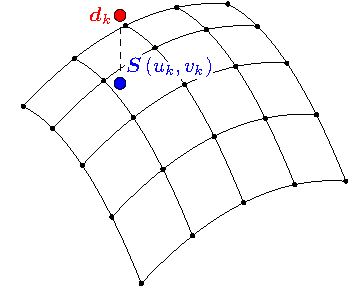
\includegraphics[scale=1]{Peters1.pdf}};
\node[] (Peters2) at ($(P2)+(-1,-.5)$){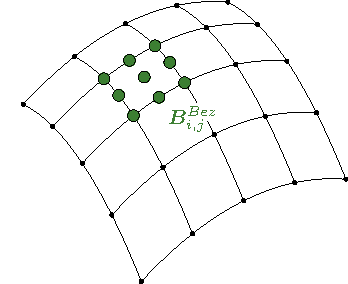
\includegraphics[scale=1]{Peters2.pdf}};
\node[] (Peters3) at ($(P3)+(-1,-.5)+(-1,-.5)$) {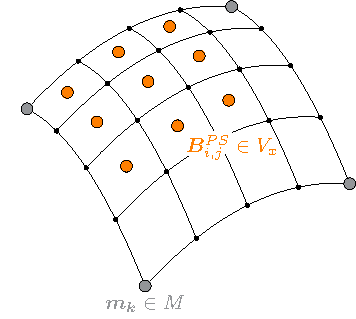
\includegraphics[scale=1]{Peters3.pdf}};
\node[circle,draw,align=center] (Peters4) at ($(P4)+(-.5,-.5)+(-1,-.5)+(-1,-.5)$) {Least squares \\ fitting \\ \scriptsize $ \norm{\lsDataPointMatrix - \lsControlPointCoefMatrix(\vec{u},\vec{v})\lsControlPointMatrix}^2$};

\draw[->,>=stealth',auto]
([yshift=-1cm]Peters1.north east) to [out=45,in=45] node[align=center]{Bernstein polynomials \\ give coefficients $c\left(u_k,v_k\right)$} ([xshift=-1cm]Peters2.north east);
\draw[->,>=stealth',auto]
([yshift=-1cm]Peters2.north east) to [out=45,in=45] node[align=center]{Peters' scheme \\ gives coefficients $C^{PS}$}([xshift=-1cm]Peters3.north east);
\draw[->,>=stealth',auto]
([yshift=-1cm]Peters3.north east) to [out=0,in=45] node[align=center]{\textbf{text1} \\ \scriptsize think about useful text here?} ([xshift=.5cm,yshift=.5cm]Peters4.north east);

\draw[->,>=stealth',auto]
([yshift=0cm,xshift=-1cm]Peters4.south west) to [out=-135,in=-135] node[align=center]{\textbf{text2} \\ \scriptsize think about useful text here.} ([yshift=1cm,xshift=1cm]Peters3.south west);
\draw[->,>=stealth',auto]
([yshift=2cm]Peters3.south west) to [out=-160,in=-135] node[align=center]{\textbf{text3} \\ \scriptsize think about useful text here?} ([yshift=1cm,xshift=1cm]Peters2.south west);
\draw[->,>=stealth',auto]
([yshift=2cm]Peters2.south west) to [out=-160,in=-135] node[align=center]{Control points $\vec{p}_{i,j}$ \\ give $\vec{S}\left(u_k,v_k\right)$} ([yshift=1cm,xshift=1cm]Peters1.south west);
\end{tikzpicture}

\end{document}